\documentclass{article}
\usepackage[utf8]{inputenc}
\usepackage[margin=1in]{geometry}
\usepackage{amsmath}
\usepackage{graphicx}
\setlength{\parindent}{0em}
\setlength{\parskip}{0.5em}


\title{CTA200 2020 Assignment 3}
\author{Henri Lamarre}
\date{}

\begin{document}

\maketitle

\section{Observed fast radio burst dispersion measures}
We begin by downloading the list of published fast radio 
burst properties from http://frbcat.org/ (described in 
https://arxiv.org/pdf/1601.03547.pdf). \\
Then, we plot the FRBs as a function of their galactic 
coordinates and colour them by their dispersion measure (DM) [left]. 
Then, we remove the estimated dispersion created by the galactic disc from the measured DM [Right].


\begin{figure}[h]
  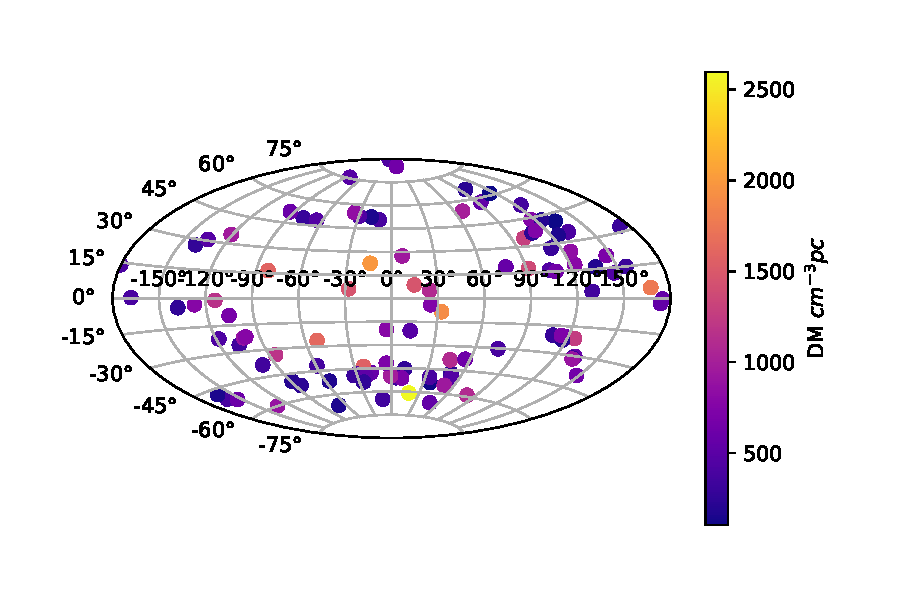
\includegraphics[width = 0.5\columnwidth]{FRB_gal_coord.pdf}
  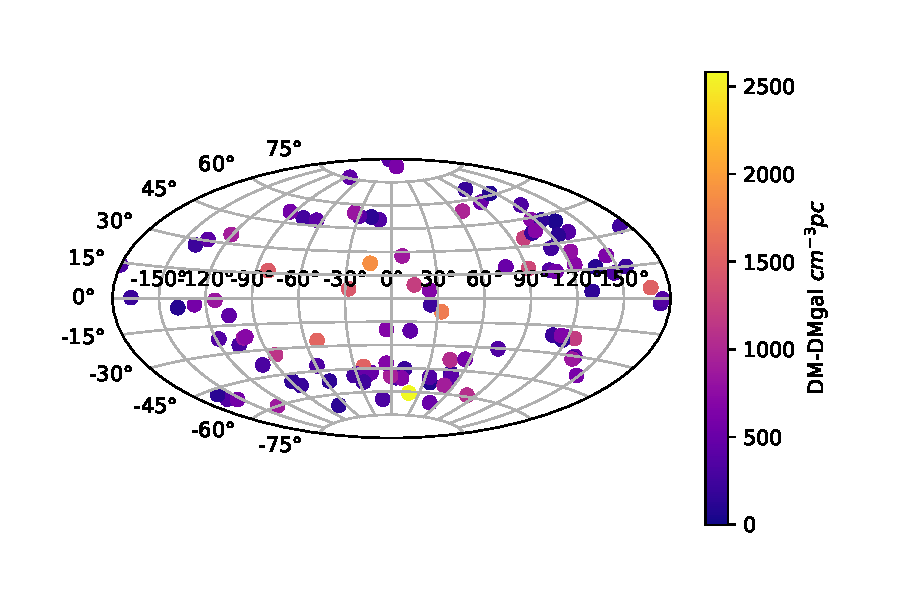
\includegraphics[width = 0.5\columnwidth]{FRB_gal_coord_corrected.pdf}
\caption{Classification of measured FRBs by their galactic coordinates and total dispersion measure (DM) [Left] and corrected dispersion measure 
(DM-D$\text{M}_\text{gal}$) [Right]. Some FRBs have a very high DM even though they don't pass through the disc of the Galaxy (yellow dot). 
This could be explained by the FRB travelling through other galaxy discs; either the host galaxy or other ones in its path.}
\label{frbcoords}
\end{figure}


\begin{figure}[h]
\begin{center}
  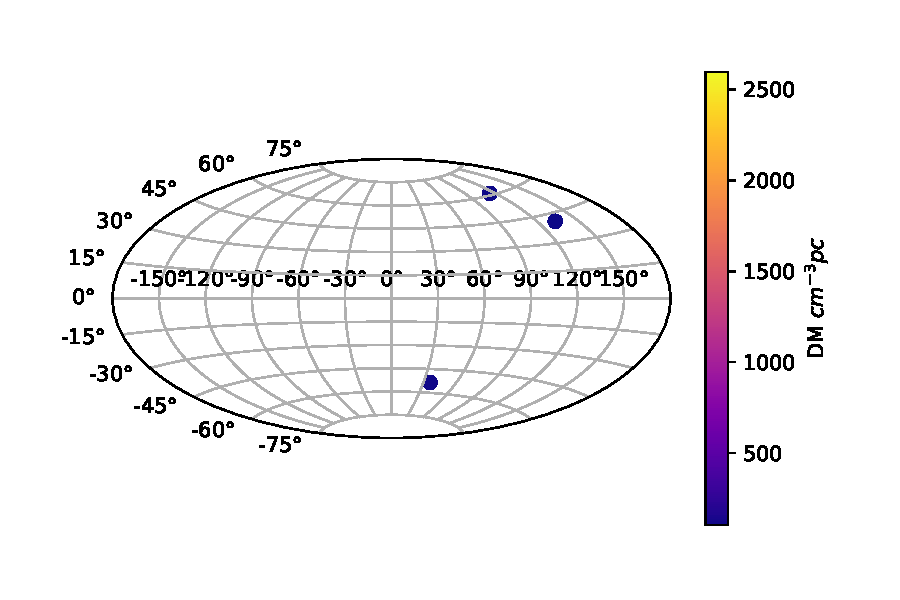
\includegraphics[width = 0.4\columnwidth]{FRB_gal_low_DM.pdf}
\caption{Three FRBs have a total DM $<120 cm^{-3}pc$. Notice that they are outside of the galactic disk. This makes sense as the dispersion measure is proportional to the number of electrons encountered by the signal and the electron density is less dense outside of the galactic disc.}
\end{center}
\end{figure}

\section{Calculating dispersion measures in the FIRE simulations}
First, we load the m12c\_res56000 data from the FIRE simulations. Then, we inspect the galaxy nested in the first halo of the corresponding halo catalog. We use trident to create a light ray that passes from the center of the halo to the radius of the galaxy, along the plane of the galaxy disc.

\begin{figure}[h]
\begin{center}
  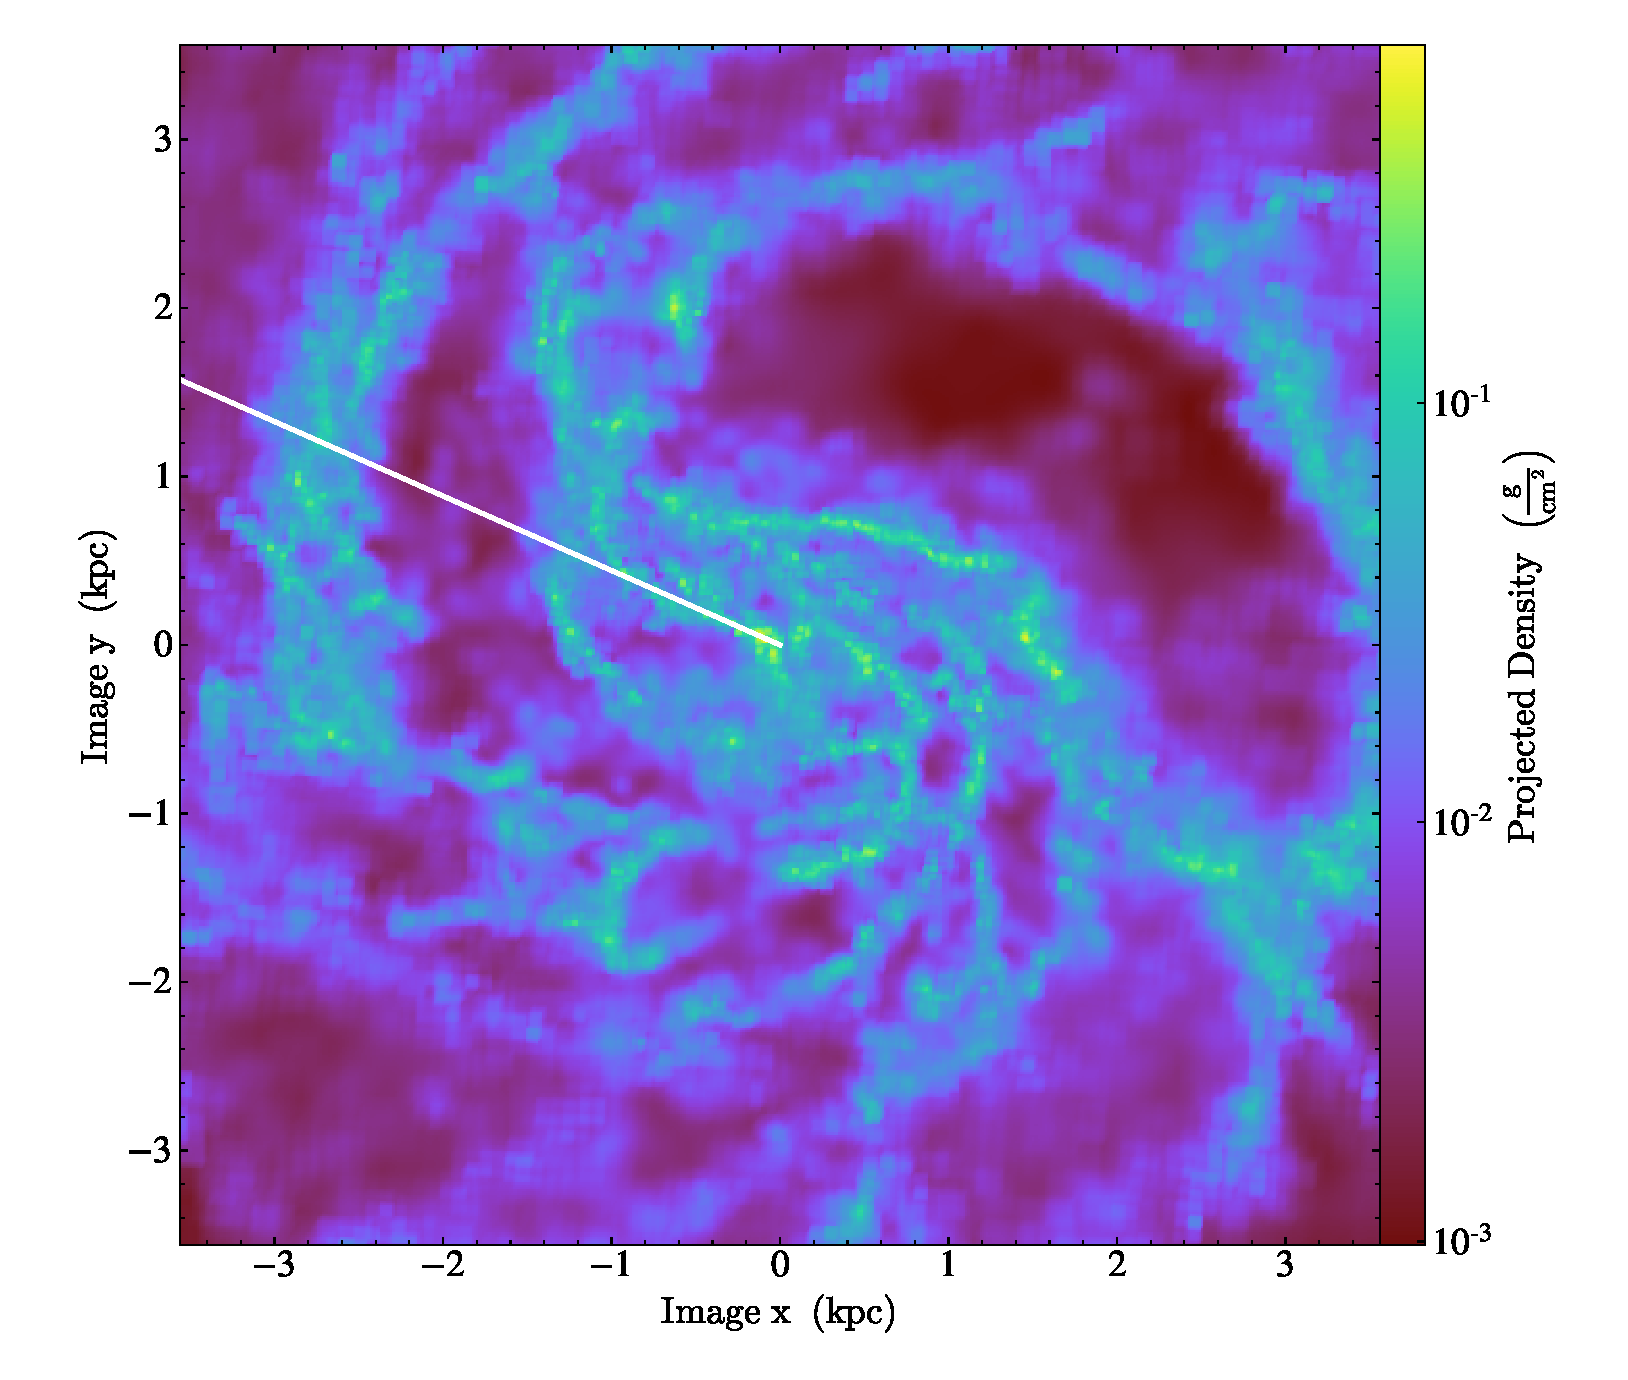
\includegraphics[width = 0.4\columnwidth]{ray_parr_galaxy.pdf}
\caption{Here, we project the density field of the galaxy such that the average angular momentum vector is perpendicular to the plot. We see in white the path of the light ray.}
\label{galaxydisc}
\end{center}
\end{figure}

\begin{figure}[h]
\begin{center}
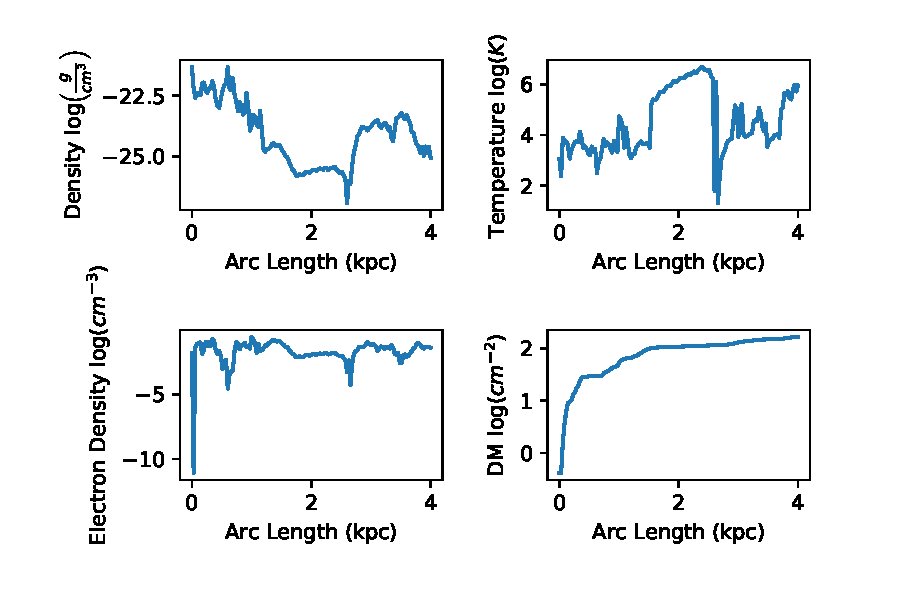
\includegraphics[width = 0.7\columnwidth]{ray_parr_subplots.pdf}
\caption{[TOP LEFT] Density field encountered by the light ray. [TOP RIGHT] Temperature field encountered by the light ray. [BOTTOM LEFT] Electron density field encountered by the light ray. [BOTTOM RIGHT] Dispersion measure computed as the line integral of the electron density along the light ray.}
\label{parsubplots}
\end{center}
\end{figure}
\newpage


Then, we do the same process with a light ray that passes from the center of the galaxy to a distance equal to the virial radius of the galaxy in the direction perpendicular to the galaxy disc.

\begin{figure}[h]
\begin{center}
  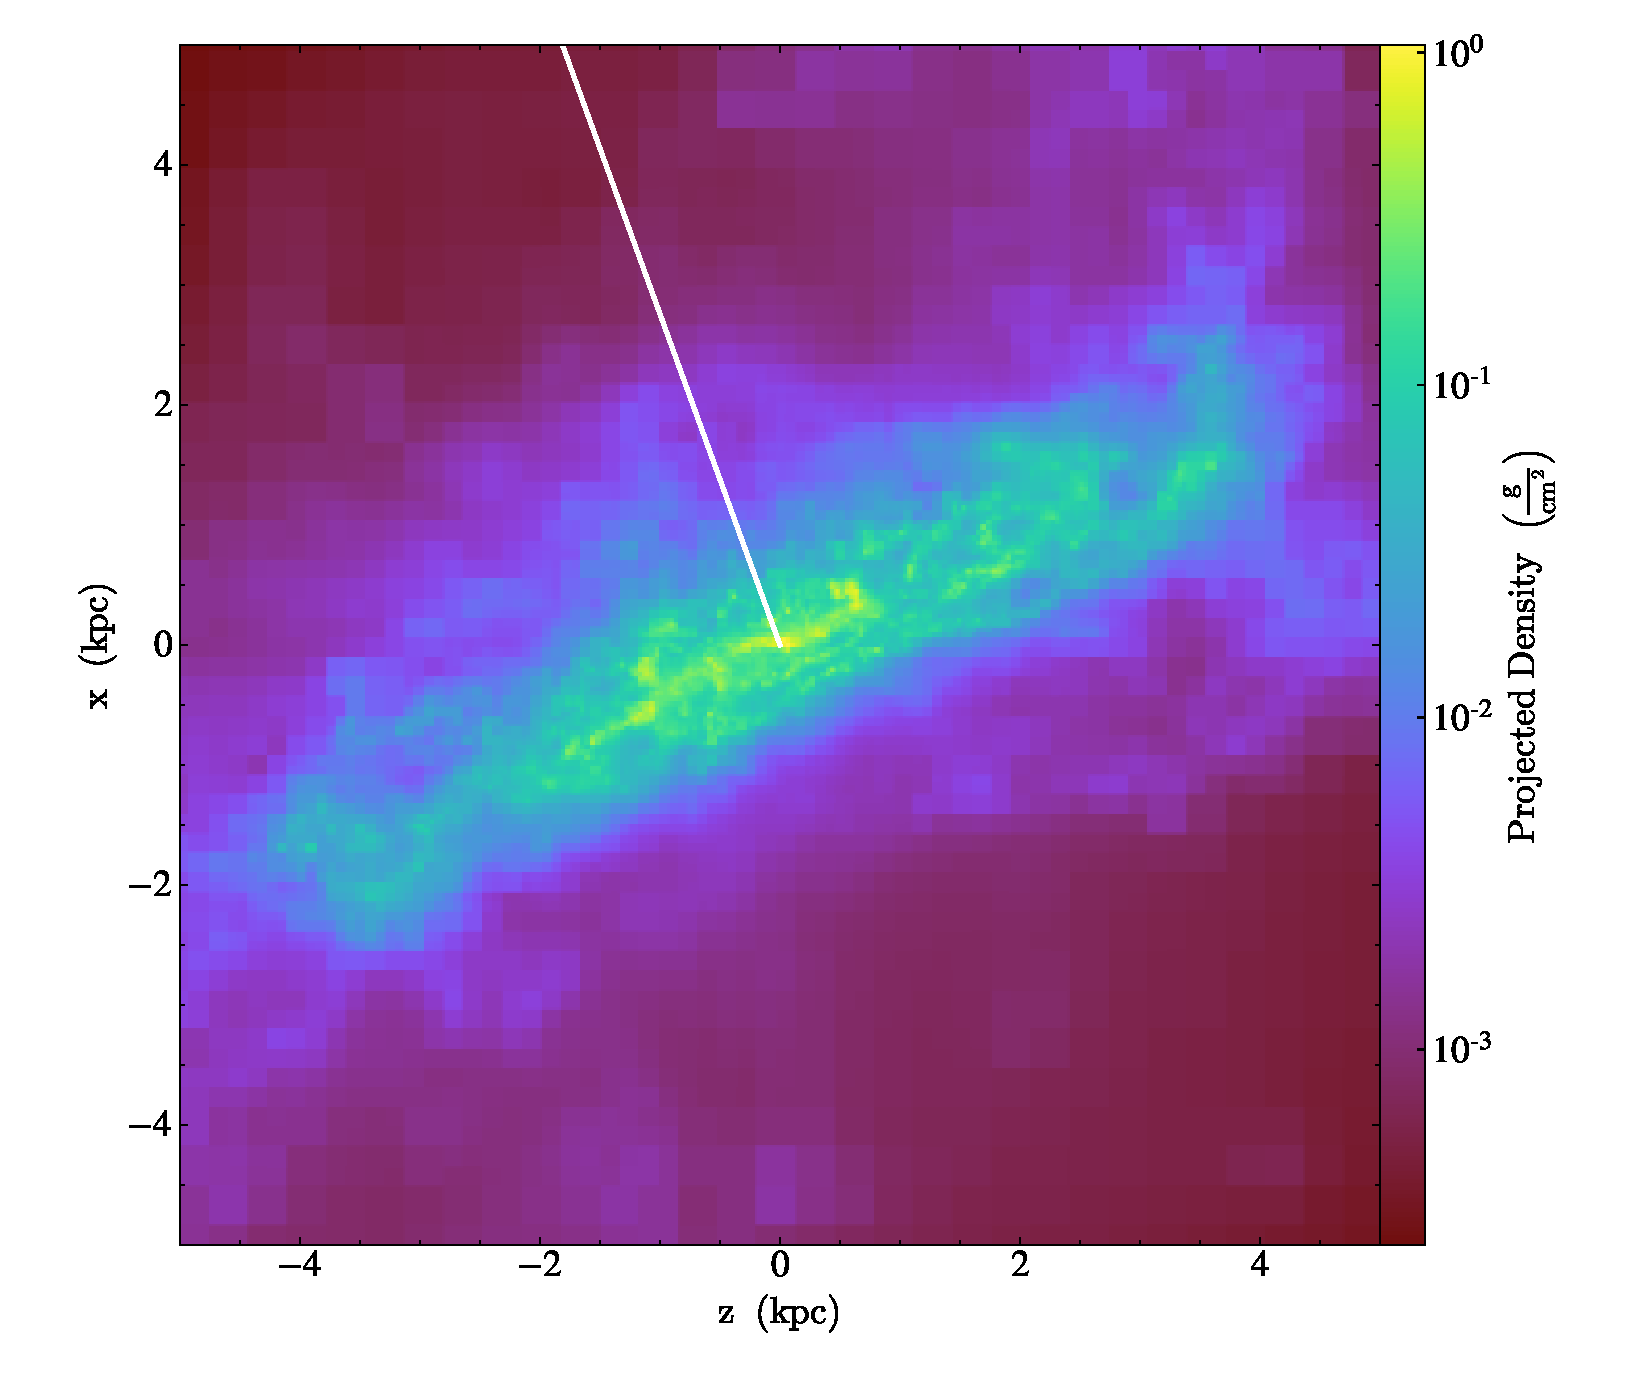
\includegraphics[width = 0.4\columnwidth]{ray_perp_galaxy_y}
\caption{Projection of the galaxy where the 'y' axis in the simulation is perpendicular to the plot. We see in white the path of the light ray.}
\label{galaxyperp}
\end{center}
\end{figure}

\begin{figure}[h]
\begin{center}
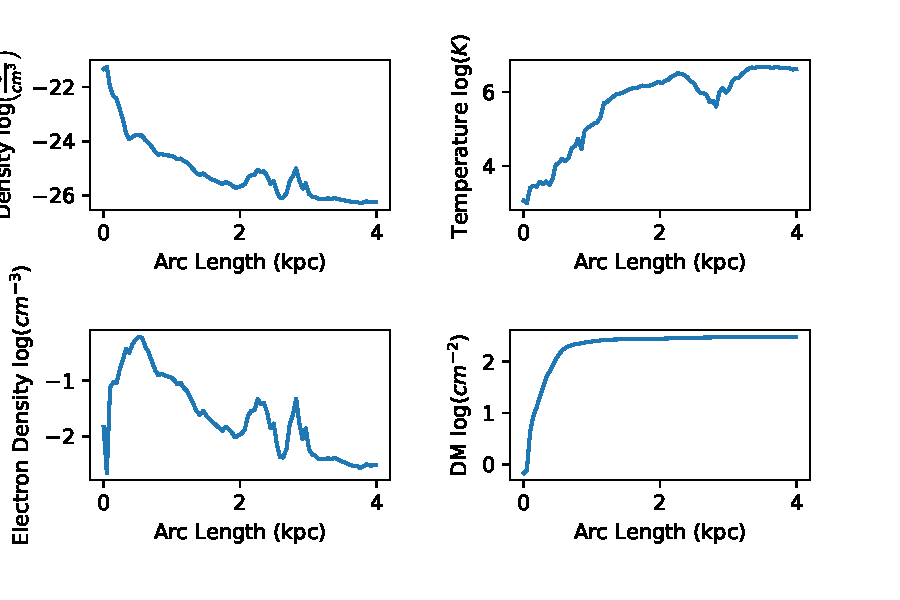
\includegraphics[width = 0.7\columnwidth]{ray_perp_subplots.pdf}
\caption{[TOP LEFT] Density field encountered by the light ray. [TOP RIGHT] Temperature field encountered by the light ray. [BOTTOM LEFT] Electron density field encountered by the light ray. [BOTTOM RIGHT] Dispersion measure computed as the line integral of the electron density along the light ray.}
\label{perpsubplots}
\end{center}
\end{figure}

Notice that the DM in figure \ref{perpsubplots} is larger than in figure \ref{parsubplots} which is unexpected as we would think that a light ray going throught the galactic plane encounters more electrons. This can be explained by the electron denisty contribution at low arclengths (from 0 to 2) which is larger for the perpendicular light ray. In other words, the gas density in the middle of the galaxy might not be only disc-shaped and a light ray perpendicular to the galaxy could in principle encounter more electrons than a ray parallel to the galaxy plane.
\end{document}
